\documentclass[../main.tex]{subfiles}

\begin{document}
\textbf{Circles and Disks}
The circle is the set of all points that have the same distance (called radius of the circle) from a given point (called center of the circle).

If $(x,y)$ is a point on a circle with center $(a,b)$ and radius $r$ then
\[
  \sqrt{(x-a)^2+(y-b)^2} = r \implies
  (x-a)^2+(y-b)^2 = r^2
\]

\begin{example}
  Find the center and radius of the circle $x^2+y^2-4x+6y=3$.

  Solution. Complete to squares to get $(x-2)^2+(y+3)^2=16$.
\end{example}

The equation $(x-a)^2+(y-b)^2 < r^2$ represents open disk and the equation $(x-a)^2+(y-b)^2 \le r^2$ represents closed disk or simply disk.
\begin{example}
  Draw $x^2+2x+y^2 \le 8$.
\end{example}
A \textbf{parabola} P is the set of all points in the plane that are equidistant from a given line L (called directrix of P) and a point F (called the focus of P).
\begin{center}
  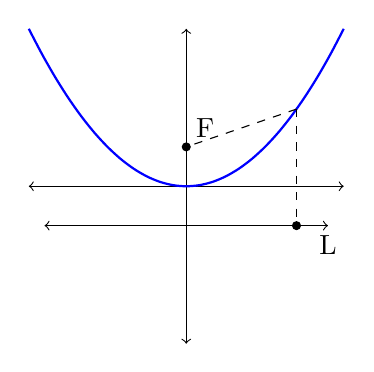
\begin{tikzpicture}[scale=2]
    \draw[<->] (-1,0)--(1,0);
    \draw[<->] (0,-1)--(0,1);
    \draw[domain=-1:1,smooth,variable=\x,blue, thick] plot ({\x},{\x*\x});
    \draw[<->] (-0.9, -0.25) -- (0.9,-0.25);
    \draw[dashed] (0.7, 0.49) -- (0.7, -0.25);
    \draw[dashed] (0.7, 0.49) -- (0, 0.25);
    \node[below] at (0.9, -0.25) {L};
    \node[above right] at (0, 0.25) {F};
    \draw[fill] (0, 0.25) circle [radius=0.025];
    \draw[fill] (0.7, -0.25) circle [radius=0.025];
    \end{tikzpicture}
\end{center}

\begin{example}
  Find the equation of the parabola having the point $F(0,p)$as focus and the line L with equation $y=-p$ as directrix.

  Solution. If $P(x,y)$ is any point on the parabola then squaring both sides of PF=PQ we get
  \[
    x^2 + (y-p)^2 = 0^2 + (y+p)^2
  \]
  After simplifying, $y=x^2/4p$.
\end{example}

\textbf{Shifting a Graph}
Let $c>0$.

\begin{itemize}
  \item To shift a graph $c$ units to the right, replace $x$ in its equation with $x-c$. To shift to left, replace $x$ by $x+c$.

  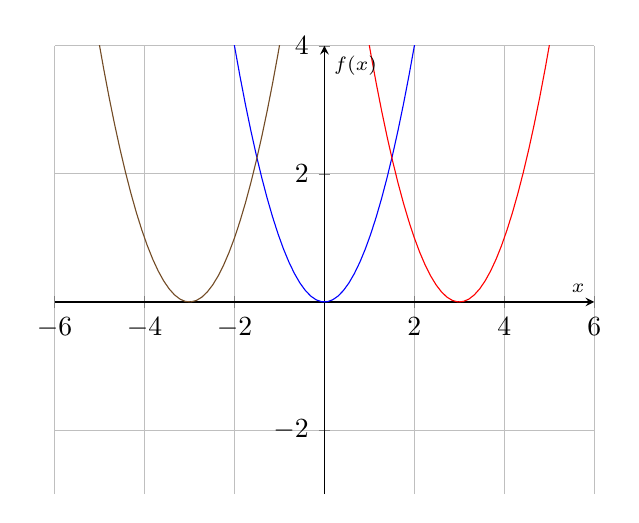
\begin{tikzpicture}
    \begin{axis}%
      [
        grid=major,
        xmin=-6,
        xmax=6,
        xlabel={\scriptsize $x$},
        axis x line=middle,
        ymin=-3,
        ymax=4,
        ylabel={\scriptsize $f(x)$},
        axis y line=middle,
        no markers,
        samples=100,
        domain=-6:6,
      ]
      \addplot (x,{x^2});
      \addplot (x,{(x-3)^2});
      \addplot (x,{(x+3)^2});
    \end{axis}
  \end{tikzpicture}
\end{itemize}


\end{document}